% Chapter 14j: Selective Energy Dysfunction Hypothesis
% Comprehensive treatment with mathematical rigor

\section{Selective Energy Dysfunction Hypothesis}
\label{sec:selective-dysfunction}

\begin{open_question}[Why Does Hair Grow Normally in Severe ME/CFS?]
A patient with severe ME/CFS cannot walk to the bathroom, cannot sustain a conversation, cannot tolerate light or sound---yet their hair continues to grow at a normal rate. Their nails grow. Wounds heal. These clinical observations, while not formally quantified in the literature, pose a fundamental challenge to the ``global energy failure'' model of ME/CFS: if mitochondrial dysfunction were truly systemic, \emph{all} energy-dependent processes should be impaired proportionally.

This chapter proposes that ME/CFS represents \emph{selective} rather than global energy dysfunction---specifically, a CNS coordination failure that impairs demand-responsive, CNS-dependent processes while sparing autonomous local processes that operate independently of central regulation.
\end{open_question}

\subsection{Motivation and Clinical Observations}

The selective dysfunction hypothesis emerged from a simple observation: processes that require CNS coordination and scale with demand are severely impaired in ME/CFS, while processes that operate autonomously at the local tissue level remain intact.

\begin{keypoint}[Preserved vs. Impaired Processes]
\textbf{Preserved} (minimal CNS dependency):
\begin{itemize}
    \item Hair growth---local follicle autonomous cycle
    \item Nail growth---keratinocyte autonomous proliferation
    \item Basic wound healing---local inflammatory cascade
    \item Baseline digestion---enteric nervous system (``second brain'')
\end{itemize}

\textbf{Severely impaired} (high CNS dependency):
\begin{itemize}
    \item Exercise capacity---requires CNS motor coordination + autonomic scaling
    \item Cognitive function---intrinsically CNS-dependent
    \item Orthostatic regulation---requires real-time CNS autonomic control
    \item Temperature regulation---hypothalamic coordination
    \item Sleep architecture---brainstem and cortical orchestration
\end{itemize}
\end{keypoint}

This pattern suggests that ME/CFS pathophysiology may preferentially affect the CNS's ability to coordinate systemic responses, rather than causing uniform cellular energy failure throughout the body.


\subsection{Formal Framework}

We formalize the selective dysfunction hypothesis using three quantitative definitions that enable testable predictions.

\begin{definition}[CNS-Dependency Index]
\label{def:cns-dependency}
For any biological process $P$, define the \textbf{CNS-dependency index} $\delta_{CNS}(P) \in [0,1]$ as:
\[
\delta_{CNS}(P) = \frac{N_{CNS}(P)}{N_{total}(P)}
\]
where $N_{CNS}(P)$ is the number of regulatory signals requiring CNS coordination and $N_{total}(P)$ is the total number of regulatory signals controlling process $P$.

\begin{itemize}
    \item $\delta_{CNS} = 0$: Fully autonomous (no CNS involvement)
    \item $\delta_{CNS} = 1$: Fully CNS-dependent (all regulation via CNS)
    \item $\delta_{CNS} \in (0,1)$: Mixed regulation
\end{itemize}
\end{definition}

\begin{definition}[Demand-Responsiveness Index]
\label{def:demand-responsiveness}
For process $P$, define the \textbf{demand-responsiveness index} $\rho(P) \in [0, \infty)$ as:
\[
\rho(P) = \frac{\max_{\text{challenge}} \text{Output}(P) - \text{Output}_{\text{baseline}}(P)}{\text{Output}_{\text{baseline}}(P)}
\]
where:
\begin{itemize}
    \item $\rho = 0$: Constant output (no demand scaling)
    \item $\rho > 0$: Output increases under challenge
    \item $\rho > 1$: Output can more than double under maximal demand
\end{itemize}

For standardization to $[0,1]$, we use $\tilde{\rho}(P) = \frac{\rho(P)}{1 + \rho(P)}$.

\textbf{Note on negative demand-response:} Some processes \emph{decrease} output under challenge (e.g., digestive function during fight-or-flight response, where blood flow diverts to skeletal muscle). For such processes, we define $\rho(P) = 0$ because the selective dysfunction hypothesis specifically addresses \emph{upregulation capacity}---the ability to increase output when demanded. Processes with negative demand-response represent regulatory suppression rather than capacity limitation, and require separate modeling frameworks (not within this hypothesis).
\end{definition}

\begin{definition}[Selective Dysfunction Severity]
\label{def:dysfunction-severity}
The \textbf{predicted dysfunction severity} for process $P$ in ME/CFS is:
\[
S(P) = \alpha \cdot \delta_{CNS}(P) + \beta \cdot \tilde{\rho}(P) + \gamma \cdot \delta_{CNS}(P) \cdot \tilde{\rho}(P)
\]
where:
\begin{itemize}
    \item $\alpha > 0$: Weight for CNS-dependency (main effect)
    \item $\beta > 0$: Weight for demand-responsiveness (main effect)
    \item $\gamma > 0$: Weight for interaction (synergistic vulnerability)
\end{itemize}

The interaction term $\gamma \cdot \delta_{CNS} \cdot \tilde{\rho}$ captures synergistic vulnerability: processes that are \emph{both} CNS-dependent \emph{and} demand-responsive are predicted to be most severely affected.
\end{definition}

\begin{hypothesis}[Selective Dysfunction Hypothesis]
\label{hyp:selective-dysfunction}
In ME/CFS, dysfunction severity $S_{observed}(P)$ correlates strongly with predicted severity $S(P)$:
\[
S_{observed}(P) = S(P) + \epsilon
\]
where $\epsilon$ is normally distributed error with mean zero.

\textbf{Testable prediction:} Spearman correlation $\rho_s$ between $S(P)$ and $S_{observed}(P)$ across processes should satisfy $\rho_s > 0.7$ (strong positive correlation).

\textbf{Falsification criterion:} If $\rho_s < 0.3$, the hypothesis is refuted.

\textbf{Certainty:} 0.55 (moderate evidence from clinical observations, formal testing required)
\end{hypothesis}


\subsection{Evidence Taxonomy}

Table~\ref{tab:process-classification} classifies biological processes by their predicted and observed dysfunction status.

\begin{table}[htbp]
\centering
\small
\caption{Process classification by CNS-dependency and demand-responsiveness with predicted and observed dysfunction in ME/CFS.}
\label{tab:process-classification}
\begin{tabular}{lccccc}
\toprule
\textbf{Process} & $\delta_{CNS}$ & $\tilde{\rho}$ & \textbf{Predicted $S$} & \textbf{Observed} & \textbf{Certainty} \\
\midrule
\multicolumn{6}{l}{\textit{Preserved processes (low $\delta_{CNS}$, low $\rho$)}} \\
Hair growth & 0.1 & 0.0 & 0.06 & Preserved & 0.7 \\
Nail growth & 0.1 & 0.0 & 0.06 & Preserved & 0.7 \\
Wound healing (basic) & 0.2 & 0.2 & 0.24 & Preserved & 0.6 \\
Digestion (baseline) & 0.3 & 0.2 & 0.30 & Variable & 0.5 \\
\midrule
\multicolumn{6}{l}{\textit{Impaired processes (high $\delta_{CNS}$ and/or high $\rho$)}} \\
Exercise capacity & 0.8 & 0.8 & 1.14 & Severe & 0.9 \\
Cognitive function & 1.0 & 0.5 & 1.05 & Severe & 0.9 \\
Orthostatic regulation & 0.9 & 0.7 & 1.14 & Severe & 0.85 \\
Temperature regulation & 0.8 & 0.4 & 0.81 & Moderate-Severe & 0.7 \\
Sleep architecture & 0.9 & 0.3 & 0.80 & Severe & 0.8 \\
Immune response to challenge & 0.5 & 0.7 & 0.79 & Dysregulated & 0.65 \\
\bottomrule
\end{tabular}

\vspace{0.3cm}
\footnotesize
\textbf{Notes:} $S$ calculated with $\alpha = 0.6$, $\beta = 0.5$, $\gamma = 0.4$. Values $>1.0$ indicate severe predicted dysfunction (additive model without upper bound). Certainty reflects confidence in classification based on literature review.
\end{table}

\begin{observation}[Demand-Response Failure Pattern]
\label{obs:demand-response}
ME/CFS patients consistently show \emph{preserved baseline function} with \emph{impaired challenge response}:
\begin{itemize}
    \item Orthostatic challenge: 91--100\% show abnormal CBF reduction during tilt-table testing, with 3-fold greater reduction than controls~\cite{Novak2022}
    \item Exercise challenge: 2-day CPET reveals decline on day 2 (vs. improvement in controls)
    \item Cognitive challenge: Fatigue elevated 24--48h post-cognitive task
\end{itemize}

This pattern is diagnostic: baseline function is maintained, but the system cannot scale to meet increased demand. This is precisely what the selective dysfunction model predicts for high-$\rho$ processes.
\end{observation}


\subsection{Causal Structure}

Figure~\ref{fig:selective-dysfunction-dag} presents the causal directed acyclic graph (DAG) for selective dysfunction. The key structural feature is the \emph{absence} of causal paths from the CNS energy crisis node to preserved autonomous processes.

\begin{figure}[htbp]
\centering
% Figure: Selective Energy Dysfunction Causal DAG
% Master causal structure showing CNS-specific energy failure with certainty-weighted edges

\begin{figure}[htbp]
\centering
\begin{tikzpicture}[
    node distance=2.2cm,
    scale=0.8, every node/.style={scale=0.8},
    % Node styles by compartment
    trigger/.style={draw=blue!70!black, fill=blue!10, very thick, rounded corners, text width=2.8cm, align=center, minimum height=1cm},
    cns/.style={draw=red!70!black, fill=red!15, very thick, rounded corners, text width=3cm, align=center, minimum height=1cm},
    cns-primary/.style={draw=red!50!black, fill=red!25, ultra thick, rounded corners, text width=3.2cm, align=center, minimum height=1.1cm, drop shadow},
    autonomic/.style={draw=orange!70!black, fill=orange!10, very thick, rounded corners, text width=2.8cm, align=center, minimum height=1cm},
    peripheral/.style={draw=purple!70!black, fill=purple!10, very thick, rounded corners, text width=2.8cm, align=center, minimum height=1cm},
    preserved/.style={draw=green!70!black, fill=green!15, very thick, rounded corners, text width=2.5cm, align=center, minimum height=0.9cm},
    % Edge styles by certainty
    high-cert/.style={-latex, very thick, black, line width=1.4pt},
    med-cert/.style={-latex, thick, gray!70!black, line width=1.1pt},
    low-cert/.style={-latex, dashed, gray!50!black, line width=0.9pt},
    no-edge/.style={-latex, dotted, gray!30!black, line width=0.7pt},
    % Labels
    cert-label/.style={font=\scriptsize\bfseries, fill=white, inner sep=1pt},
]

% Title
\node[font=\large\bfseries] at (0, 10) {Selective Energy Dysfunction: Causal Structure};

% === TRIGGERS (top) ===
\begin{scope}[yshift=7cm]
    \node[trigger] (infection) at (-4, 0) {\textbf{Viral Infection}\\Post-infectious onset};
    \node[trigger] (stress) at (0, 0) {\textbf{Severe Stress}\\Physiological/psychological};
    \node[trigger] (immune) at (4, 0) {\textbf{Immune Dysregulation}\\Autoantibodies, cytokines};
\end{scope}

% === PRIMARY DYSFUNCTION (CNS Energy Crisis) ===
\node[cns-primary] (cns-crisis) at (0, 4.5) {\textbf{CNS ENERGY CRISIS}\\Brain hypometabolism\\Catecholamine deficit};

% Trigger arrows
\draw[high-cert] (infection) -- (cns-crisis) node[cert-label, midway, left] {0.7};
\draw[med-cert] (stress) -- (cns-crisis) node[cert-label, midway, right] {0.5};
\draw[high-cert] (immune) -- (cns-crisis) node[cert-label, midway, right] {0.65};

% === DOWNSTREAM CNS EFFECTS ===
\begin{scope}[yshift=1.5cm]
    \node[cns] (cognitive) at (-4, 0) {\textbf{Cognitive Dysfunction}\\Brain fog, memory\\Executive function};
    \node[cns] (autonomic-ctrl) at (0, 0) {\textbf{Autonomic Control Failure}\\Impaired signaling\\Coordination loss};
    \node[cns] (neuroendocrine) at (4, 0) {\textbf{Neuroendocrine Disruption}\\HPA axis\\Circadian rhythm};
\end{scope}

% CNS crisis to downstream
\draw[high-cert] (cns-crisis) -- (cognitive) node[cert-label, midway, above left] {0.85};
\draw[high-cert] (cns-crisis) -- (autonomic-ctrl) node[cert-label, midway, right] {0.8};
\draw[med-cert] (cns-crisis) -- (neuroendocrine) node[cert-label, midway, above right] {0.6};

% === AUTONOMIC/PERIPHERAL CASCADE ===
\begin{scope}[yshift=-1.5cm]
    \node[autonomic] (oi) at (-3, 0) {\textbf{Orthostatic Intolerance}\\POTS, CBF reduction\\3-fold vs controls};
    \node[peripheral] (exercise) at (1.5, 0) {\textbf{Exercise Intolerance}\\PEM, 2-day CPET\\Demand-response failure};
    \node[autonomic] (temperature) at (5, 0) {\textbf{Temperature Dysregulation}\\Thermostat impaired};
\end{scope}

% Autonomic control to periphery
\draw[high-cert] (autonomic-ctrl) -- (oi) node[cert-label, midway, left] {0.75};
\draw[med-cert] (autonomic-ctrl) -- (exercise) node[cert-label, midway, right] {0.65};
\draw[med-cert] (neuroendocrine) -- (temperature) node[cert-label, midway, right] {0.55};

% Cross-connections
\draw[low-cert, bend right=20] (oi) to node[cert-label, below] {0.4} (cognitive);

% === PRESERVED AUTONOMOUS PROCESSES (bottom right, unconnected) ===
\begin{scope}[xshift=7cm, yshift=-1cm]
    \node[preserved] (hair) at (0, 2) {\textbf{Hair Growth}\\Normal rate\\$\delta_{CNS} = 0.1$};
    \node[preserved] (nails) at (0, 0.5) {\textbf{Nail Growth}\\Normal rate\\$\delta_{CNS} = 0.1$};
    \node[preserved] (wound) at (0, -1) {\textbf{Wound Healing}\\Preserved\\$\delta_{CNS} = 0.2$};

    % Box around preserved
    \node[draw=green!50!black, dashed, thick, rounded corners, fit=(hair)(nails)(wound), inner sep=8pt, label={[font=\small\bfseries, green!50!black]above:PRESERVED}] {};
\end{scope}

% === NO CONNECTION from CNS to preserved (explicit) ===
\draw[no-edge] (cns-crisis.east) -- ++(1.5,0) node[cert-label, above, gray!50!black] {$\times$ No causal path} -- ++(0.5,-0.5);

% === FEEDBACK LOOPS ===
\draw[low-cert, bend left=40] (exercise.south) to node[cert-label, below] {0.35} (cns-crisis.south);
\node[font=\tiny\itshape, text width=2cm, align=center] at (-1, 0.3) {PEM worsens\\CNS state};

% === LEGEND ===
\begin{scope}[yshift=-4.5cm, xshift=-4cm]
    \node[font=\small\bfseries] at (0, 0.8) {Edge Certainty (0--1 scale):};
    \draw[high-cert] (0, 0.3) -- (1.5, 0.3) node[right, font=\small] {High ($\geq 0.7$): Strong evidence};
    \draw[med-cert] (0, -0.2) -- (1.5, -0.2) node[right, font=\small] {Medium (0.5--0.7): Moderate evidence};
    \draw[low-cert] (0, -0.7) -- (1.5, -0.7) node[right, font=\small] {Low ($< 0.5$): Limited/speculative};
\end{scope}

% === COMPARTMENT LEGEND ===
\begin{scope}[yshift=-4.5cm, xshift=4cm]
    \node[font=\small\bfseries] at (0, 0.8) {Compartments:};
    \node[cns, minimum width=1.5cm, minimum height=0.5cm, font=\tiny] at (0.5, 0.3) {CNS};
    \node[font=\small, right] at (1.3, 0.3) {Central nervous system};
    \node[autonomic, minimum width=1.5cm, minimum height=0.5cm, font=\tiny] at (0.5, -0.2) {Auto};
    \node[font=\small, right] at (1.3, -0.2) {Autonomic regulation};
    \node[preserved, minimum width=1.5cm, minimum height=0.5cm, font=\tiny] at (0.5, -0.7) {Pres};
    \node[font=\small, right] at (1.3, -0.7) {Autonomous/preserved};
\end{scope}

% === KEY INSIGHT BOX ===
\node[draw=black!70, fill=yellow!5, rounded corners, text width=13cm, align=left, font=\small, inner sep=8pt] at (0, -7) {
\textbf{Key Structural Feature:} The CNS energy crisis node has \emph{no causal path} to autonomous processes (hair, nails, wound healing). These processes operate via local autonomous regulation with minimal CNS coordination ($\delta_{CNS} < 0.2$). Their preservation despite severe ME/CFS symptoms supports the selective dysfunction hypothesis: the disease targets CNS-dependent, demand-responsive processes while sparing CNS-independent autonomous functions.
};

\end{tikzpicture}
\caption{Causal structure of selective energy dysfunction in ME/CFS. Edge weights indicate certainty (0--1 scale) based on evidence quality. The absence of edges to preserved processes (green) demonstrates selective targeting of CNS-dependent functions.}
\label{fig:selective-dysfunction-dag}
\end{figure}

\end{figure}

The DAG encodes the following causal claims with certainty-weighted edges:

\begin{enumerate}
    \item \textbf{Triggers $\rightarrow$ CNS Energy Crisis} (certainty: 0.65--0.70): Viral infection, immune dysregulation, or severe stress initiates CNS energy deficit
    \item \textbf{CNS Crisis $\rightarrow$ Cognitive Dysfunction} (certainty: 0.85): Direct effect of brain hypometabolism
    \item \textbf{CNS Crisis $\rightarrow$ Autonomic Control Failure} (certainty: 0.80): Impaired CNS signaling disrupts autonomic regulation
    \item \textbf{Autonomic Failure $\rightarrow$ Orthostatic Intolerance} (certainty: 0.75): Secondary to failed cardiovascular coordination
    \item \textbf{No edge: CNS $\rightarrow$ Autonomous Processes}: Hair, nails, wound healing operate independently
\end{enumerate}


\subsection{Mechanistic Sub-Hypotheses}

Five mechanistic hypotheses explain \emph{why} CNS might be selectively vulnerable.

\subsubsection{Astrocyte Energy Gate Hypothesis}

The astrocyte-neuron lactate shuttle (ANLS) provides 30--50\% of neuronal ATP~\cite{Pellerin1994,Magistretti2018}. Unlike peripheral tissues with direct glucose access, neurons depend on astrocytes to convert glucose to lactate and shuttle it via monocarboxylate transporters (MCT2/MCT4).

\begin{hypothesis}[Astrocyte Energy Gate]
\label{hyp:astrocyte-gate}
Dysfunction in the astrocyte-neuron lactate shuttle causes CNS-specific energy failure while peripheral tissues (with direct glucose access) remain unaffected.

\textbf{Mechanism:}
\begin{align}
L_n &= k_{MCT} \cdot [L_a] \cdot f(\text{transporter integrity}) \\
E_n &= g(L_n, \text{mitochondrial function})
\end{align}
where $L_n$ = neuronal lactate uptake, $L_a$ = astrocyte lactate concentration, $k_{MCT}$ = MCT transporter efficiency, $E_n$ = neuronal ATP production.

\textbf{ME/CFS hypothesis:} Reduced $k_{MCT}$ or impaired $f(\cdot)$ $\Rightarrow$ $L_n \downarrow$ despite normal $L_a$ $\Rightarrow$ CNS-specific energy deficit.

\textbf{Certainty:} 0.4 (plausible mechanism from neuroscience; no direct ME/CFS evidence)
\end{hypothesis}

Figure~\ref{fig:astrocyte-lactate-shuttle} illustrates the ANLS mechanism and proposed dysfunction site.

\begin{figure}[htbp]
\centering
% Figure: Astrocyte-Neuron Lactate Shuttle (ANLS) Dysfunction
% Shows proposed mechanism for CNS-specific energy failure

\begin{figure}[htbp]
\centering
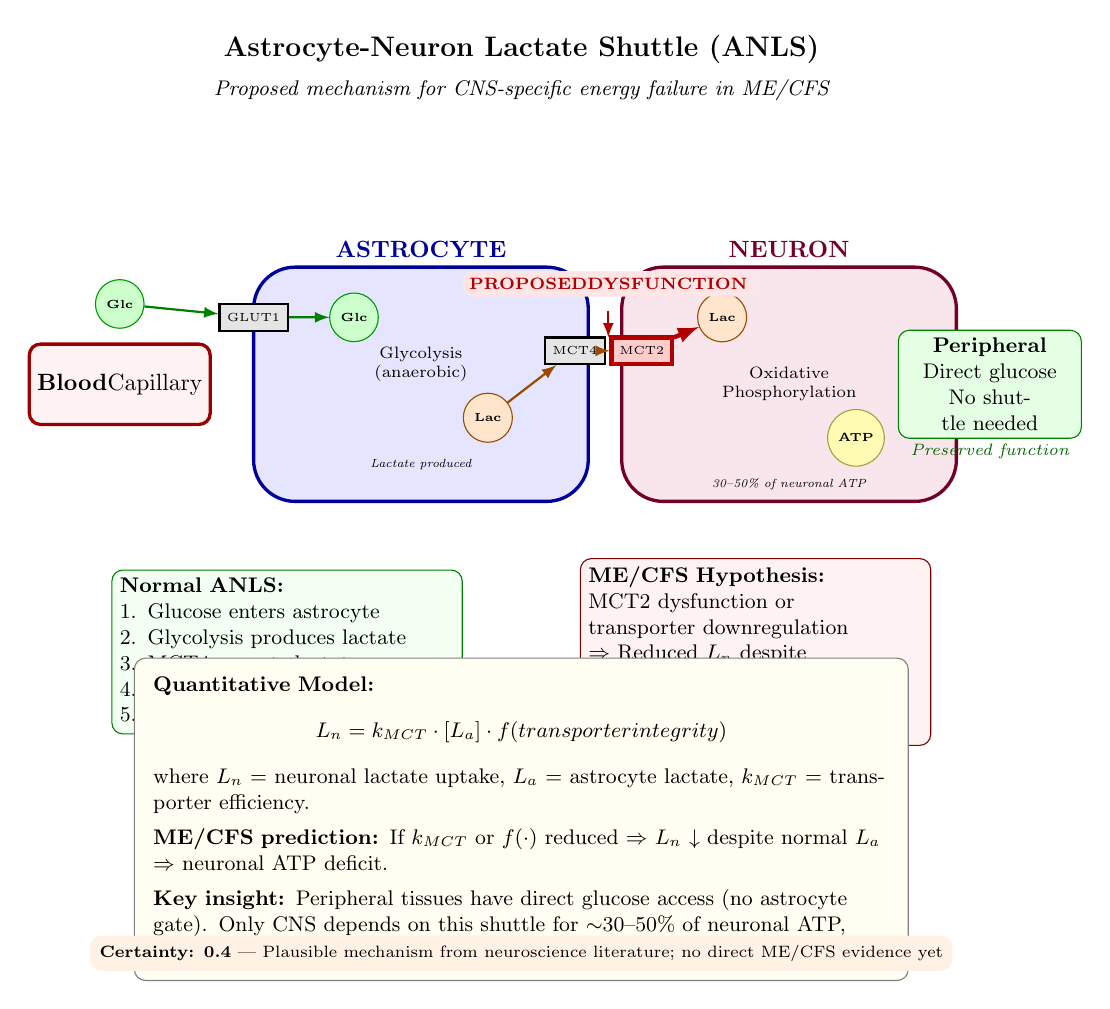
\begin{tikzpicture}[
    scale=0.85, every node/.style={scale=0.85},
    % Cell styles
    astrocyte/.style={draw=blue!60!black, fill=blue!10, very thick, rounded corners=15pt, minimum width=5cm, minimum height=3.5cm},
    neuron/.style={draw=purple!60!black, fill=purple!10, very thick, rounded corners=15pt, minimum width=5cm, minimum height=3.5cm},
    capillary/.style={draw=red!60!black, fill=red!5, very thick, rounded corners, minimum width=2cm, minimum height=1.2cm},
    % Molecule styles
    glucose/.style={circle, draw=green!60!black, fill=green!20, minimum size=0.6cm, font=\tiny\bfseries},
    lactate/.style={circle, draw=orange!60!black, fill=orange!20, minimum size=0.6cm, font=\tiny\bfseries},
    atp/.style={circle, draw=yellow!60!black, fill=yellow!30, minimum size=0.6cm, font=\tiny\bfseries},
    % Transporter styles
    transporter/.style={draw=black, fill=gray!20, thick, minimum width=0.8cm, minimum height=0.4cm, font=\tiny},
    transporter-impaired/.style={draw=red!70!black, fill=red!20, ultra thick, minimum width=0.8cm, minimum height=0.4cm, font=\tiny},
    % Arrow styles
    flow/.style={-latex, thick, green!50!black},
    flow-impaired/.style={-latex, very thick, red!70!black, dashed},
    shuttle/.style={-latex, thick, orange!60!black},
    shuttle-impaired/.style={-latex, ultra thick, red!70!black, dashed},
]

% Title
\node[font=\large\bfseries] at (0, 8) {Astrocyte-Neuron Lactate Shuttle (ANLS)};
\node[font=\small\itshape] at (0, 7.4) {Proposed mechanism for CNS-specific energy failure in ME/CFS};

% === BLOOD CAPILLARY ===
\node[capillary] (cap) at (-6, 3) {\textbf{Blood}\\Capillary};
\node[glucose] (gluc-blood) at (-6, 4.2) {Glc};

% === ASTROCYTE ===
\node[astrocyte, label={[font=\bfseries, blue!60!black]above:ASTROCYTE}] (astro) at (-1.5, 3) {};

% Astrocyte contents
\node[glucose] (gluc-astro) at (-2.5, 4) {Glc};
\node[font=\scriptsize, text width=2cm, align=center] at (-1.5, 3.3) {Glycolysis\\(anaerobic)};
\node[lactate] (lac-astro) at (-0.5, 2.5) {Lac};
\node[font=\tiny\itshape] at (-1.5, 1.8) {Lactate produced};

% Glucose transporter (BBB to astrocyte)
\node[transporter] (glut1) at (-4, 4) {GLUT1};
\draw[flow] (gluc-blood) -- (glut1);
\draw[flow] (glut1) -- (gluc-astro);

% === NEURON ===
\node[neuron, label={[font=\bfseries, purple!60!black]above:NEURON}] (neur) at (4, 3) {};

% Neuron contents
\node[lactate] (lac-neur) at (3, 4) {Lac};
\node[font=\scriptsize, text width=2cm, align=center] at (4, 3) {Oxidative\\Phosphorylation};
\node[atp] (atp-neur) at (5, 2.2) {ATP};
\node[font=\tiny\itshape] at (4, 1.5) {30--50\% of neuronal ATP};

% === MCT TRANSPORTERS (key site) ===
% Astrocyte MCT4 (lactate export)
\node[transporter] (mct4) at (0.8, 3.5) {MCT4};
\draw[shuttle] (lac-astro) -- (mct4);

% Neuron MCT2 (lactate import) - POTENTIALLY IMPAIRED
\node[transporter-impaired] (mct2) at (1.8, 3.5) {MCT2};
\draw[shuttle] (mct4) -- (mct2);
\draw[shuttle-impaired] (mct2) -- (lac-neur);

% Impairment indicator
\node[font=\scriptsize\bfseries, red!70!black, fill=red!10, rounded corners, inner sep=3pt] at (1.3, 4.5) {PROPOSED\\DYSFUNCTION};
\draw[-latex, red!70!black, thick] (1.3, 4.1) -- (1.3, 3.7);

% === NORMAL PATHWAY ANNOTATION ===
\begin{scope}[yshift=-1cm]
    \node[draw=green!50!black, fill=green!5, rounded corners, text width=5cm, align=left, font=\small] at (-3.5, 0) {
    \textbf{Normal ANLS:}\\
    1. Glucose enters astrocyte\\
    2. Glycolysis produces lactate\\
    3. MCT4 exports lactate\\
    4. MCT2 imports to neuron\\
    5. Oxidative phos. $\rightarrow$ ATP
    };
\end{scope}

% === ME/CFS HYPOTHESIS ANNOTATION ===
\begin{scope}[yshift=-1cm]
    \node[draw=red!50!black, fill=red!5, rounded corners, text width=5cm, align=left, font=\small] at (3.5, 0) {
    \textbf{ME/CFS Hypothesis:}\\
    MCT2 dysfunction or\\
    transporter downregulation\\
    $\Rightarrow$ Reduced $L_n$ despite\\
    \hspace{6pt} normal $L_a$\\
    $\Rightarrow$ CNS-specific energy\\
    \hspace{6pt} deficit
    };
\end{scope}

% === EQUATIONS ===
\node[draw=black!50, fill=yellow!5, rounded corners, text width=11cm, align=left, font=\small, inner sep=8pt] at (0, -3.5) {
\textbf{Quantitative Model:}
\[
L_n = k_{MCT} \cdot [L_a] \cdot f(\text{transporter integrity})
\]
where $L_n$ = neuronal lactate uptake, $L_a$ = astrocyte lactate, $k_{MCT}$ = transporter efficiency.\\[4pt]
\textbf{ME/CFS prediction:} If $k_{MCT}$ or $f(\cdot)$ reduced $\Rightarrow$ $L_n \downarrow$ despite normal $L_a$ $\Rightarrow$ neuronal ATP deficit.\\[4pt]
\textbf{Key insight:} Peripheral tissues have direct glucose access (no astrocyte gate). Only CNS depends on this shuttle for $\sim$30--50\% of neuronal ATP, explaining CNS-specific vulnerability.
};

% === PERIPHERAL COMPARISON ===
\begin{scope}[xshift=7cm, yshift=3cm]
    \node[draw=green!50!black, fill=green!10, rounded corners, text width=2.5cm, align=center, font=\small] (periph) at (0, 0) {\textbf{Peripheral}\\Direct glucose\\No shuttle needed};
    \node[font=\scriptsize\itshape, green!40!black] at (0, -1) {Preserved function};
\end{scope}

% === CERTAINTY ===
\node[font=\scriptsize, fill=orange!10, rounded corners, inner sep=4pt] at (0, -5.5) {
\textbf{Certainty: 0.4} --- Plausible mechanism from neuroscience literature; no direct ME/CFS evidence yet
};

\end{tikzpicture}
\caption{Astrocyte-neuron lactate shuttle (ANLS) as proposed mechanism for CNS-specific energy dysfunction. If MCT2 transporter function is impaired, neurons cannot access lactate-derived ATP while peripheral tissues (with direct glucose access) remain unaffected.}
\label{fig:astrocyte-lactate-shuttle}
\end{figure}

\end{figure}


\subsubsection{CNS Energy Triage Hypothesis}

Under energy scarcity, the CNS may implement a hardwired priority hierarchy that preserves vital functions at the expense of ``luxury'' cognitive processes.

\begin{hypothesis}[CNS Energy Triage]
\label{hyp:energy-triage}
The CNS implements a priority-based energy allocation system under scarcity:
\begin{enumerate}
    \item \textbf{Tier 1} (never sacrificed): Brainstem vital functions --- $E_{min} = 0.30 \cdot E_{total}$
    \item \textbf{Tier 2}: Sensory processing --- $E_{threshold} = 0.50 \cdot E_{total}$
    \item \textbf{Tier 3}: Motor coordination --- $E_{threshold} = 0.60 \cdot E_{total}$
    \item \textbf{Tier 4}: Memory consolidation --- $E_{threshold} = 0.70 \cdot E_{total}$
    \item \textbf{Tier 5}: Executive function --- $E_{threshold} = 0.85 \cdot E_{total}$
    \item \textbf{Tier 6} (first sacrificed): Complex cognition --- $E_{threshold} = 0.95 \cdot E_{total}$
\end{enumerate}

\textbf{Prediction:} Cognitive symptoms should follow the inverse hierarchy. Complex cognition fails first; vital functions never fail.

\textbf{Clinical correlation:} ``Brain fog'' (executive dysfunction, Tier 5--6) is among the earliest and most prominent symptoms, consistent with these tiers being sacrificed first.

\textbf{Certainty:} 0.5 (consistent with observed symptom hierarchy; formal testing needed)
\end{hypothesis}

Figure~\ref{fig:energy-triage-hierarchy} visualizes the triage hierarchy with the typical ME/CFS energy threshold.

\begin{figure}[htbp]
\centering
% Figure: CNS Energy Triage Hierarchy
% Shows priority levels for CNS functions under energy scarcity

\begin{figure}[htbp]
\centering
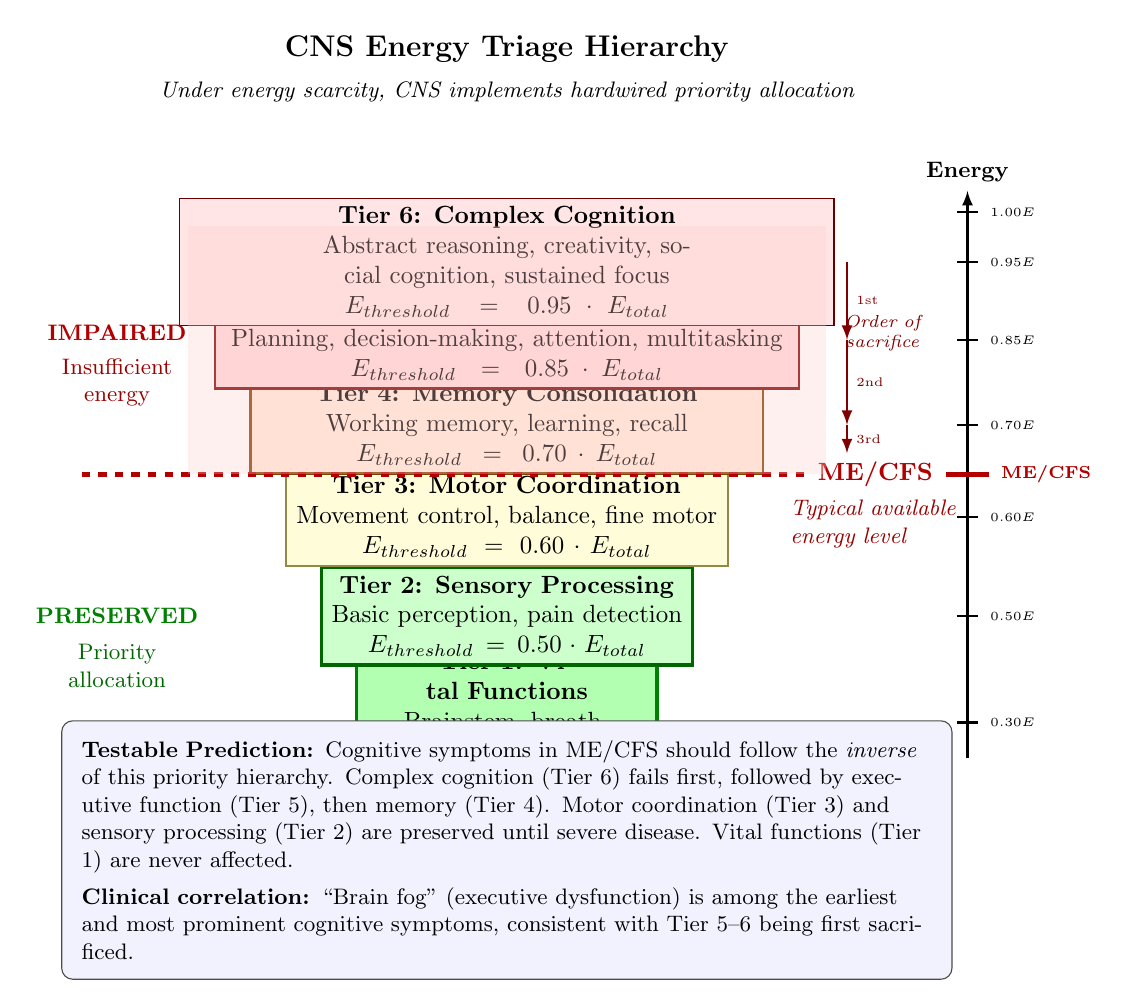
\begin{tikzpicture}[
    scale=0.9, every node/.style={scale=0.9},
    % Tier styles (darker = higher priority)
    tier1/.style={draw=green!50!black, fill=green!30, very thick, text width=4cm, align=center, minimum height=1.2cm},
    tier2/.style={draw=green!40!black, fill=green!20, very thick, text width=5cm, align=center, minimum height=1.1cm},
    tier3/.style={draw=yellow!50!black, fill=yellow!15, thick, text width=6cm, align=center, minimum height=1cm},
    tier4/.style={draw=orange!50!black, fill=orange!15, thick, text width=7cm, align=center, minimum height=1cm},
    tier5/.style={draw=red!50!black, fill=red!15, thick, text width=8cm, align=center, minimum height=1cm},
    tier6/.style={draw=red!40!black, fill=red!10, text width=9cm, align=center, minimum height=0.9cm},
    % Energy line
    energy-line/.style={ultra thick, dashed, red!70!black},
    % Threshold labels
    threshold/.style={font=\scriptsize\bfseries, fill=white, inner sep=2pt},
]

% Title
\node[font=\large\bfseries] at (0, 9.5) {CNS Energy Triage Hierarchy};
\node[font=\small\itshape] at (0, 8.9) {Under energy scarcity, CNS implements hardwired priority allocation};

% === PYRAMID TIERS (bottom to top = highest to lowest priority) ===

% Tier 1: Vital (never sacrificed)
\node[tier1] (t1) at (0, 0) {\textbf{Tier 1: Vital Functions}\\Brainstem, breathing, cardiac rhythm\\$E_{min} = 0.30 \cdot E_{total}$};

% Tier 2: Critical
\node[tier2] (t2) at (0, 1.5) {\textbf{Tier 2: Sensory Processing}\\Basic perception, pain detection\\$E_{threshold} = 0.50 \cdot E_{total}$};

% Tier 3: Important
\node[tier3] (t3) at (0, 2.9) {\textbf{Tier 3: Motor Coordination}\\Movement control, balance, fine motor\\$E_{threshold} = 0.60 \cdot E_{total}$};

% Tier 4: Standard
\node[tier4] (t4) at (0, 4.2) {\textbf{Tier 4: Memory Consolidation}\\Working memory, learning, recall\\$E_{threshold} = 0.70 \cdot E_{total}$};

% Tier 5: Non-essential
\node[tier5] (t5) at (0, 5.4) {\textbf{Tier 5: Executive Function}\\Planning, decision-making, attention, multitasking\\$E_{threshold} = 0.85 \cdot E_{total}$};

% Tier 6: Luxury
\node[tier6] (t6) at (0, 6.5) {\textbf{Tier 6: Complex Cognition}\\Abstract reasoning, creativity, social cognition, sustained focus\\$E_{threshold} = 0.95 \cdot E_{total}$};

% === ME/CFS ENERGY LINE ===
\draw[energy-line] (-6, 3.5) -- (6, 3.5);
\node[font=\bfseries, red!70!black, fill=white, inner sep=3pt] at (5.2, 3.5) {ME/CFS};
\node[font=\small\itshape, red!60!black, text width=3cm, align=left] at (5.5, 2.8) {Typical available\\energy level};

% === SHADING FOR AFFECTED TIERS ===
\fill[red!20, opacity=0.3] (-4.5, 3.5) rectangle (4.5, 7);

% Labels for affected vs preserved
\node[font=\small\bfseries, red!70!black] at (-5.5, 5.5) {IMPAIRED};
\node[font=\small, red!60!black, text width=2cm, align=center] at (-5.5, 4.8) {Insufficient energy};

\node[font=\small\bfseries, green!50!black] at (-5.5, 1.5) {PRESERVED};
\node[font=\small, green!40!black, text width=2cm, align=center] at (-5.5, 0.8) {Priority allocation};

% === ENERGY SCALE (right side) ===
\begin{scope}[xshift=6.5cm]
    \draw[thick, -latex] (0, -0.5) -- (0, 7.5) node[above, font=\small\bfseries] {Energy};

    % Markers
    \foreach \y/\val in {0/0.30, 1.5/0.50, 2.9/0.60, 4.2/0.70, 5.4/0.85, 6.5/0.95, 7.2/1.00} {
        \draw[thick] (-0.15, \y) -- (0.15, \y);
        \node[right, font=\tiny] at (0.2, \y) {$\val E$};
    }

    % ME/CFS marker
    \draw[red!70!black, ultra thick] (-0.3, 3.5) -- (0.3, 3.5);
    \node[right, font=\scriptsize\bfseries, red!70!black] at (0.35, 3.5) {ME/CFS};
\end{scope}

% === PREDICTION BOX ===
\node[draw=black!70, fill=blue!5, rounded corners, text width=12cm, align=left, font=\small, inner sep=8pt] at (0, -1.8) {
\textbf{Testable Prediction:} Cognitive symptoms in ME/CFS should follow the \emph{inverse} of this priority hierarchy. Complex cognition (Tier 6) fails first, followed by executive function (Tier 5), then memory (Tier 4). Motor coordination (Tier 3) and sensory processing (Tier 2) are preserved until severe disease. Vital functions (Tier 1) are never affected.\\[4pt]
\textbf{Clinical correlation:} ``Brain fog'' (executive dysfunction) is among the earliest and most prominent cognitive symptoms, consistent with Tier 5--6 being first sacrificed.
};

% === ARROWS showing sacrifice order ===
\draw[-latex, thick, red!50!black] (4.8, 6.5) -- (4.8, 5.4) node[midway, right, font=\tiny] {1st};
\draw[-latex, thick, red!50!black] (4.8, 5.4) -- (4.8, 4.2) node[midway, right, font=\tiny] {2nd};
\draw[-latex, thick, red!50!black] (4.8, 4.2) -- (4.8, 3.8) node[midway, right, font=\tiny] {3rd};

\node[font=\scriptsize\itshape, red!50!black, text width=1.5cm, align=center] at (5.3, 5.5) {Order of sacrifice};

\end{tikzpicture}
\caption{CNS energy triage hierarchy under energy scarcity. The red dashed line indicates typical available energy in ME/CFS. Functions above the line (Tiers 4--6) are impaired; functions below (Tiers 1--3) are preferentially preserved through energy allocation.}
\label{fig:energy-triage-hierarchy}
\end{figure}

\end{figure}


\subsubsection{Blood-Brain Barrier Vulnerability Hypothesis}

The blood-brain barrier (BBB) creates a unique vulnerability: damage signals may accumulate in the CNS while peripheral clearance continues normally.

\begin{hypothesis}[BBB Compartmentalization]
\label{hyp:bbb-vulnerability}
The BBB traps mitochondrial damage markers and limits cofactor delivery, causing CNS-specific accumulation of dysfunction.

\textbf{Steady-state model:}
\[
\frac{[M]_{CSF}}{[M]_{blood}} = \frac{R_{production}}{P_{BBB} \cdot k_{clear}}
\]
where $[M]$ = damage marker concentration, $R_{production}$ = production rate, $P_{BBB}$ = BBB permeability, $k_{clear}$ = clearance rate.

\textbf{ME/CFS prediction:} If $P_{BBB}$ is reduced or $R_{production}$ elevated, the CSF/blood ratio increases, indicating CNS-specific accumulation.

\textbf{Testable:} Measure mtDNA, 8-OHdG, or other damage markers in paired CSF and blood samples. Elevated CSF/blood ratio supports hypothesis.

\textbf{Certainty:} 0.45 (BBB dysfunction documented in neuroinflammation; ME/CFS-specific data limited)
\end{hypothesis}


\subsubsection{Sickness Behavior Persistence Hypothesis}

Evolutionary sickness behavior programs target \emph{behavioral outputs} (requiring CNS) while sparing truly autonomous processes.

\begin{hypothesis}[Sickness Behavior Stuck On]
\label{hyp:sickness-behavior}
ME/CFS represents a sickness behavior program that fails to disengage, chronically suppressing CNS-mediated behavioral outputs while leaving autonomous local processes unaffected.

\textbf{Activation function:}
\[
\text{SB}(t) = \sigma\left(\sum_{i} w_i \cdot [\text{cytokine}_i](t) - \theta\right)
\]
where $\sigma$ is sigmoid activation, $w_i$ are cytokine weights, and $\theta$ is the activation threshold.

\textbf{Normal state:} Acute infection elevates cytokines $\Rightarrow$ SB activates $\Rightarrow$ infection resolves $\Rightarrow$ cytokines normalize $\Rightarrow$ SB deactivates.

\textbf{ME/CFS state:} Chronic low-grade immune activation maintains $\sum w_i \cdot [\text{cytokine}_i] > \theta$ indefinitely $\Rightarrow$ SB persists.

\textbf{Evolutionary logic:} Sickness behavior evolved to suppress \emph{behavioral} energy expenditure during infection. Hair growth has no behavioral component and was never targeted by this program.

\textbf{Certainty:} 0.55 (strong evolutionary logic; moderate mechanistic support from neuroimaging~\cite{Nakatomi2014neuroinflammation})
\end{hypothesis}


\subsubsection{Partial Torpor Trap Hypothesis}

ME/CFS may represent incomplete engagement of torpor-like metabolic suppression mechanisms.

\begin{hypothesis}[Partial Torpor Trap]
\label{hyp:torpor}
ME/CFS involves partial engagement of torpor/hibernation pathways with failed arousal, trapping patients in a low-metabolic state.

\textbf{Torpor engagement dynamics:}
\[
\frac{d(\text{MR})}{dt} = -\alpha \cdot T_{signal} + \beta \cdot A_{signal}
\]
where MR = metabolic rate, $T_{signal}$ = torpor induction signal, $A_{signal}$ = arousal signal.

\textbf{Normal torpor:} $\alpha \cdot T > \beta \cdot A$ during entry; $\beta \cdot A > \alpha \cdot T$ during arousal.

\textbf{ME/CFS state:} $\alpha \cdot T > \beta \cdot A$ chronically (trapped in partial suppression).

\textbf{Testable markers:} Torpor-associated molecules (H$_2$S, adenosine, orexin) may be dysregulated.

\textbf{Certainty:} 0.35 (speculative; inspired by emerging torpor biology research)
\end{hypothesis}


\subsection{Testable Predictions}

The selective dysfunction hypothesis generates specific, falsifiable predictions.

\begin{prediction}[Hair Follicle Mitochondrial Function]
\label{pred:hair-follicle}
\textbf{Hypothesis:} Hair follicle mitochondria are functionally normal in ME/CFS patients.

\textbf{Measurement:} Mitochondrial respiration (oxygen consumption rate, OCR) in plucked hair follicle cells.

\textbf{Statistical design:}
\begin{itemize}
    \item Test type: Equivalence test (TOST procedure)
    \item Equivalence margin: $\delta = 0.2 \times \bar{x}_{control}$ (20\% of control mean)
    \item Sample size: $n = 40$ per group (power = 0.8, $\alpha = 0.05$)
    \item Outcome: ME/CFS OCR equivalent to control OCR
\end{itemize}

\textbf{Interpretation:}
\begin{itemize}
    \item If confirmed: Strong support for selective (not global) mitochondrial dysfunction
    \item If refuted (ME/CFS OCR significantly lower): Global dysfunction model supported
\end{itemize}

\textbf{Feasibility:} Hair follicle collection is minimally invasive; mitochondrial respiration assays are established.
\end{prediction}

\begin{prediction}[CSF-to-Blood Lactate Gradient]
\label{pred:csf-lactate}
\textbf{Hypothesis:} CSF lactate is elevated relative to blood lactate in ME/CFS, indicating impaired lactate shuttling in CNS.

\textbf{Measurement:} Paired CSF and blood lactate concentrations.

\textbf{Statistical design:}
\begin{itemize}
    \item Test type: Two-sample $t$-test on ratio $[L]_{CSF}/[L]_{blood}$
    \item Expected effect size: Cohen's $d \geq 0.5$ (medium effect)
    \item Sample size: $n = 64$ per group (power = 0.8, $\alpha = 0.05$)
    \item Outcome: Ratio elevated in ME/CFS vs. controls
\end{itemize}

\textbf{Interpretation:}
\begin{itemize}
    \item If confirmed: Supports astrocyte energy gate hypothesis
    \item If refuted: Lactate shuttle not primary mechanism
\end{itemize}
\end{prediction}

\begin{prediction}[Peripheral ATP During PEM]
\label{pred:peripheral-atp}
\textbf{Hypothesis:} Peripheral muscle ATP is preserved during PEM crashes (dysfunction is coordination failure, not local energy deficit).

\textbf{Measurement:} $^{31}$P-MRS of skeletal muscle during provoked PEM.

\textbf{Statistical design:}
\begin{itemize}
    \item Test type: Repeated measures ANOVA (baseline vs. PEM)
    \item Expected: No significant decline in muscle ATP during PEM
    \item Comparison: CNS metabolic markers (via PET/MRS) should decline while peripheral markers remain stable
\end{itemize}

\textbf{Interpretation:}
\begin{itemize}
    \item If confirmed: Dysfunction is CNS coordination failure, not peripheral energy deficit
    \item If refuted (peripheral ATP drops): Global depletion model supported
\end{itemize}
\end{prediction}

\begin{prediction}[Direct Stimulation vs. Voluntary Contraction]
\label{pred:direct-stim}
\textbf{Hypothesis:} Direct electrical stimulation of muscles produces greater force than voluntary contraction in ME/CFS patients.

\textbf{Rationale:} If dysfunction is CNS coordination failure, bypassing CNS via direct stimulation should restore output.

\textbf{Measurement:} Compare force production: voluntary maximal contraction vs. electrical stimulation.

\textbf{Expected:} $F_{electrical} / F_{voluntary} > 1$ in ME/CFS (vs. ratio $\approx 1$ in controls).

\textbf{Interpretation:}
\begin{itemize}
    \item If confirmed: Peripheral muscle capable; CNS drive impaired
    \item If refuted: Peripheral muscle intrinsically impaired
\end{itemize}
\end{prediction}

\begin{prediction}[Cognitive Triage Hierarchy]
\label{pred:cognitive-hierarchy}
\textbf{Hypothesis:} Cognitive impairment in ME/CFS follows the inverse of the energy triage hierarchy.

\textbf{Measurement:} Cognitive battery assessing each tier:
\begin{itemize}
    \item Tier 6 (complex cognition): Abstract reasoning, creativity
    \item Tier 5 (executive function): Planning, multitasking, attention
    \item Tier 4 (memory): Working memory, recall
    \item Tier 3 (motor coordination): Fine motor, reaction time
    \item Tier 2 (sensory processing): Basic perception
\end{itemize}

\textbf{Expected:} Impairment severity: Tier 6 > Tier 5 > Tier 4 > Tier 3 > Tier 2.

\textbf{Statistical test:} Ordinal regression testing hierarchy effect.
\end{prediction}


\subsection{Subtype Classification Model}

The selective dysfunction framework suggests natural subtypes based on primary compartment affected.

\begin{hypothesis}[Selective Dysfunction Subtypes]
\label{hyp:subtypes}
ME/CFS can be classified into subtypes based on which compartment shows primary dysfunction:

\textbf{Input features (with measurement basis):}
\begin{itemize}
    \item $x_1$: CSF catecholamine deficit (z-score relative to healthy controls)
    \begin{itemize}
        \item Measurement: CSF dopamine, norepinephrine, serotonin metabolites
        \item Reference: NIH deep phenotyping study found significant CSF catecholamine reductions~\cite{walitt2024deep}
    \end{itemize}
    \item $x_2$: Orthostatic CBF reduction (\% decline from supine to upright)
    \begin{itemize}
        \item Measurement: Transcranial Doppler during tilt-table test
        \item Reference: Controls show $\sim$5--10\% reduction; ME/CFS shows $\sim$20--30\% (3-fold greater)~\cite{Novak2022}
    \end{itemize}
    \item $x_3$: Muscle ATP deficit at rest (\% below control mean)
    \begin{itemize}
        \item Measurement: $^{31}$P-MRS of quadriceps or forearm
        \item Reference: Variable findings in literature; some studies show 20--40\% reduction
    \end{itemize}
    \item $x_4$: Neuroimaging abnormality score (composite z-score)
    \begin{itemize}
        \item Measurement: PET neuroinflammation markers, fMRI activation patterns, MRS metabolites
        \item Reference: Nakatomi et al.\ found 45--199\% elevation in neuroinflammation markers~\cite{Nakatomi2014neuroinflammation}
    \end{itemize}
\end{itemize}

\textbf{Proposed classification rules (preliminary thresholds):}

The following thresholds are \emph{preliminary estimates} based on effect sizes in the literature. They require empirical validation through clustering analysis on a multi-biomarker cohort before clinical application.

\textbf{Note on units:} Thresholds use z-scores ($\sigma$) for standardized measures and absolute percentages (\%) for CBF changes, reflecting conventions in respective literatures.

\begin{align*}
\text{Subtype A (CNS-Primary)} &: x_1 < -1.5\sigma \land x_4 > 2\sigma \land x_3 > -0.5\sigma \\
&\quad \text{(CNS markers abnormal, peripheral spared)} \\[0.5em]
\text{Subtype B (Autonomic-Primary)} &: x_2 > 25\% \land x_1 > -1.0\sigma \\
&\quad \text{(OI dominant, CNS markers near-normal)} \\[0.5em]
\text{Subtype C (Peripheral-Primary)} &: x_3 < -1.5\sigma \land x_1 > -1.0\sigma \land x_4 < 1\sigma \\
&\quad \text{(Muscle deficit primary, CNS spared)} \\[0.5em]
\text{Subtype D (Global/Advanced)} &: \geq 3 \text{ of } \{x_1 < -1.5\sigma, x_2 > 25\%, x_3 < -1.5\sigma, x_4 > 2\sigma\} \\
&\quad \text{(Multi-system involvement)}
\end{align*}

\textbf{Threshold rationale:}
\begin{itemize}
    \item $-1.5\sigma$: Corresponds to approximately the 7th percentile of control distribution---outside normal variation
    \item $2\sigma$: Corresponds to approximately the 98th percentile---clearly elevated
    \item $25\%$ CBF reduction: Approximately 2.5\,$\times$ the normal orthostatic response (note: this is an absolute percentage, not a z-score, reflecting how CBF changes are typically reported in the literature)
\end{itemize}

\textbf{Overlap precedence:} When a patient meets criteria for multiple subtypes:
\begin{enumerate}
    \item If $\geq 3$ criteria met $\Rightarrow$ classify as Subtype D (Global) regardless of other matches
    \item Otherwise, assign to the subtype with the most extreme abnormality (largest z-score deviation or percentage reduction); if tied, prioritize CNS-Primary $>$ Autonomic-Primary $>$ Peripheral-Primary (reflecting the hypothesis that CNS dysfunction is upstream)
    \item Document secondary subtype features for treatment consideration
\end{enumerate}

\textbf{Validation protocol required:}
\begin{enumerate}
    \item Collect multi-biomarker panel in $n \geq 200$ ME/CFS patients (sample size rationale: with 4 subtypes and 4 input features, minimum 50 patients per subtype needed for stable cluster estimation; $n = 200$ provides robustness against unequal subtype prevalence and allows 10\% holdout for validation, with $k$-fold cross-validation to compensate for small holdout size)
    \item Perform unsupervised clustering (k-means, hierarchical) to identify natural groupings
    \item Compare data-driven clusters to proposed subtypes
    \item Calculate sensitivity/specificity for each classification rule
    \item Refine thresholds based on ROC analysis to optimize classification accuracy
\end{enumerate}

\textbf{Treatment implications (contingent on validation):}
\begin{itemize}
    \item Subtype A: CNS-penetrant compounds, intranasal delivery, neuroinflammation-targeted therapy
    \item Subtype B: Autonomic modulators (midodrine, pyridostigmine), volume expansion
    \item Subtype C: Mitochondrial support, muscle-targeted interventions, exercise rehabilitation if tolerated
    \item Subtype D: Multi-system approach, sequential targeting of dominant compartments
\end{itemize}

\textbf{Certainty:} 0.35 (framework theoretically motivated; all thresholds are preliminary estimates requiring empirical validation before any clinical application)
\end{hypothesis}


\subsection{Treatment Implications}

The selective dysfunction hypothesis has immediate treatment implications.

\subsubsection{Pharmacological Bypass Evidence}

\begin{observation}[Midodrine Effectiveness]
\label{obs:midodrine}
Midodrine (direct $\alpha_1$-adrenergic agonist) improves orthostatic symptoms in patients with POTS and orthostatic intolerance---conditions highly comorbid with ME/CFS---by directly stimulating peripheral vasculature, bypassing CNS autonomic coordination~\cite{Ojha2024pediatricPOTS}.

\textbf{Implication:} If peripheral targets were intrinsically dysfunctional, pharmacological bypass would not restore function. Midodrine effectiveness proves the peripheral machinery is intact; only CNS coordination is impaired.

This is evidence for the selective dysfunction model: the problem is signaling/coordination, not end-organ failure.
\end{observation}

\subsubsection{Therapeutic Strategy}

\begin{keypoint}[Treatment Strategy from Selective Dysfunction Model]
\begin{enumerate}
    \item \textbf{CNS-targeted delivery}: Intranasal or intrathecal routes may outperform oral for CNS-targeted compounds
    \item \textbf{Pharmacological bypass}: Direct-acting agents that bypass CNS coordination (midodrine, direct muscle stimulation)
    \item \textbf{Reduce CNS energy demands}: Pacing as CNS energy management, not just ``activity reduction''
    \item \textbf{Subtype-specific targeting}: Match intervention to primary dysfunction compartment
\end{enumerate}
\end{keypoint}


\subsection{Compartmental Energy Model}

Figure~\ref{fig:compartmental-energy-model} presents the four-compartment energy model with CNS as the coordination bottleneck.

\begin{figure}[htbp]
\centering
% Figure: Compartmental Energy Model
% Shows 4-compartment energy flow with CNS as bottleneck

\begin{figure}[htbp]
\centering
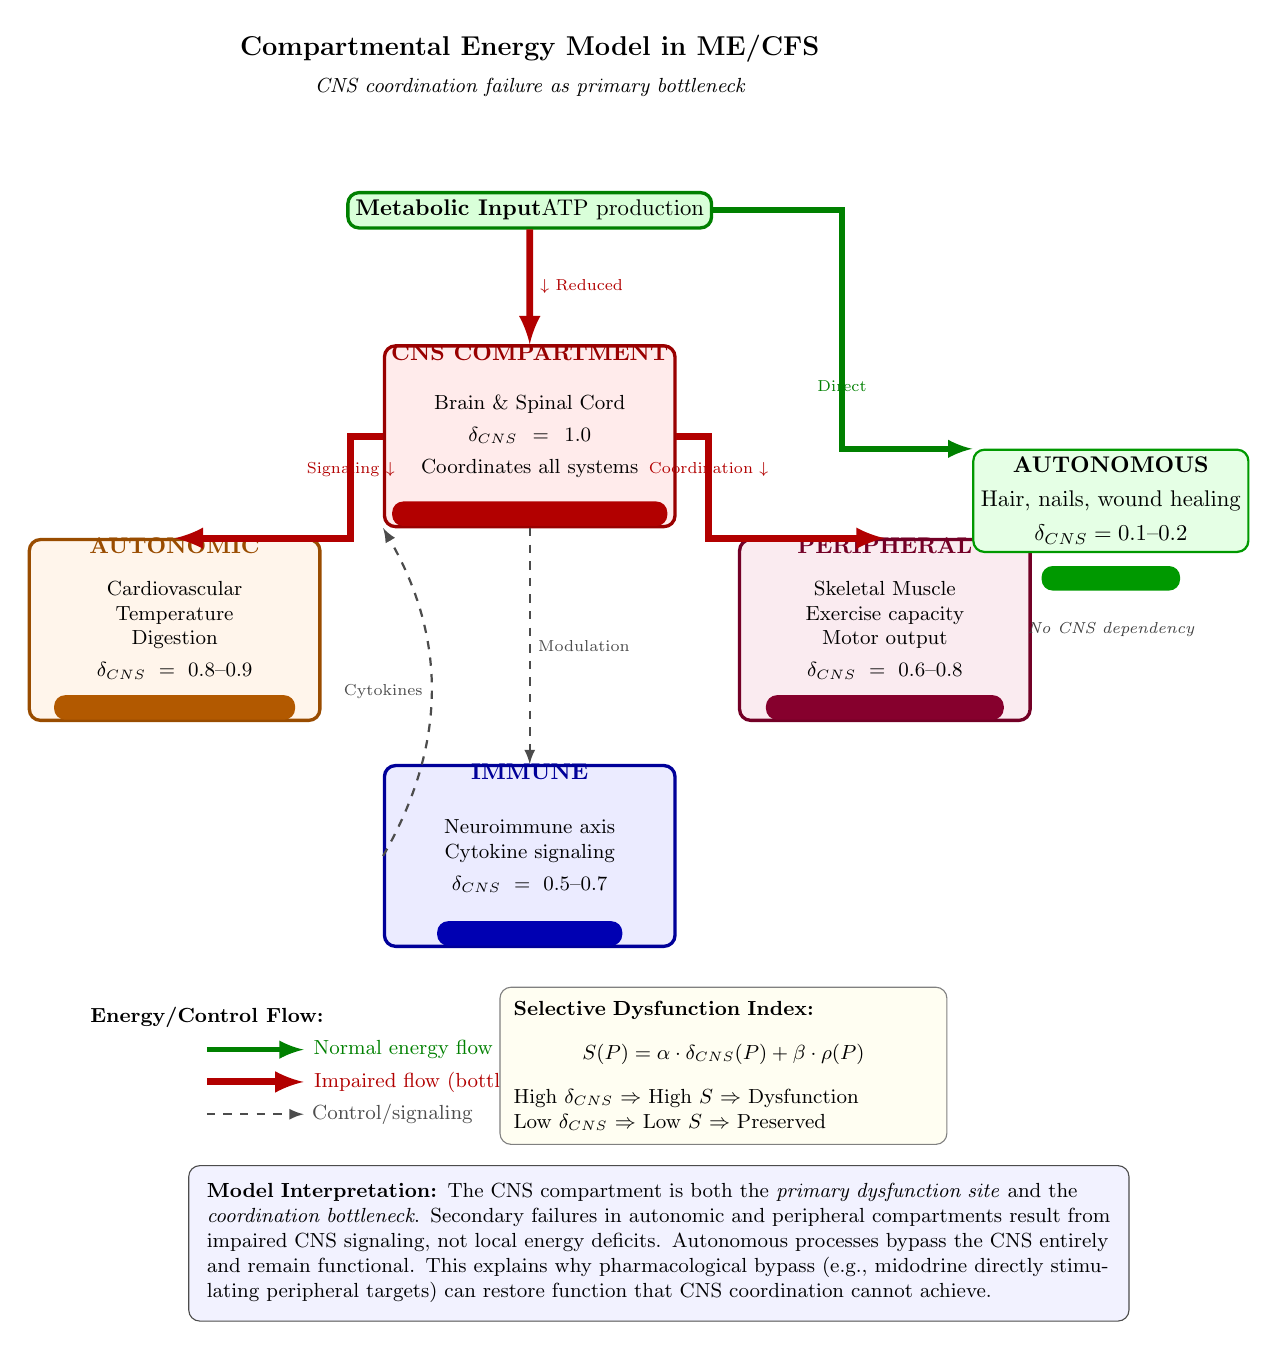
\begin{tikzpicture}[
    scale=0.82, every node/.style={scale=0.82},
    % Compartment styles
    compartment/.style={draw=black!70, very thick, rounded corners, minimum width=4.5cm, minimum height=2.8cm, align=center},
    cns-comp/.style={compartment, draw=red!60!black, fill=red!8},
    auto-comp/.style={compartment, draw=orange!60!black, fill=orange!8},
    periph-comp/.style={compartment, draw=purple!60!black, fill=purple!8},
    immune-comp/.style={compartment, draw=blue!60!black, fill=blue!8},
    preserved-comp/.style={draw=green!60!black, fill=green!10, thick, rounded corners, minimum width=3cm, minimum height=1.5cm, align=center},
    % Arrow styles
    energy-flow/.style={-latex, very thick, line width=2pt},
    control/.style={-latex, thick, dashed, gray!60!black},
    impaired/.style={-latex, ultra thick, red!70!black, line width=2.5pt},
    % Status indicators
    status/.style={font=\scriptsize\bfseries, rounded corners, inner sep=3pt},
]

% Title
\node[font=\large\bfseries] at (0, 9) {Compartmental Energy Model in ME/CFS};
\node[font=\small\itshape] at (0, 8.4) {CNS coordination failure as primary bottleneck};

% === ENERGY INPUT (top) ===
\node[draw=green!50!black, fill=green!15, very thick, rounded corners, minimum width=3cm] (input) at (0, 6.5) {\textbf{Metabolic Input}\\ATP production};

% === CNS COMPARTMENT (center, primary) ===
\node[cns-comp] (cns) at (0, 3) {};
\node[font=\bfseries, red!60!black] at (0, 4.3) {CNS COMPARTMENT};
\node[font=\small, text width=4cm, align=center] at (0, 3) {
    Brain \& Spinal Cord\\[3pt]
    $\delta_{CNS} = 1.0$\\[3pt]
    Coordinates all systems
};
\node[status, fill=red!20, red!70!black] at (0, 1.8) {PRIMARY DYSFUNCTION};

% Energy to CNS (impaired)
\draw[impaired] (input) -- (cns) node[midway, right, font=\scriptsize] {$\downarrow$ Reduced};

% === AUTONOMIC COMPARTMENT (left) ===
\node[auto-comp] (auto) at (-5.5, 0) {};
\node[font=\bfseries, orange!60!black] at (-5.5, 1.3) {AUTONOMIC};
\node[font=\small, text width=4cm, align=center] at (-5.5, 0) {
    Cardiovascular\\
    Temperature\\
    Digestion\\[3pt]
    $\delta_{CNS} = 0.8$--$0.9$
};
\node[status, fill=orange!20, orange!70!black] at (-5.5, -1.2) {SECONDARY FAILURE};

% CNS control to Autonomic (impaired)
\draw[impaired] (cns.west) -- ++(-0.5,0) |- (auto.north) node[pos=0.25, above, font=\scriptsize] {Signaling $\downarrow$};

% === PERIPHERAL COMPARTMENT (right) ===
\node[periph-comp] (periph) at (5.5, 0) {};
\node[font=\bfseries, purple!60!black] at (5.5, 1.3) {PERIPHERAL};
\node[font=\small, text width=4cm, align=center] at (5.5, 0) {
    Skeletal Muscle\\
    Exercise capacity\\
    Motor output\\[3pt]
    $\delta_{CNS} = 0.6$--$0.8$
};
\node[status, fill=purple!20, purple!70!black] at (5.5, -1.2) {COORDINATION LOSS};

% CNS control to Peripheral (impaired)
\draw[impaired] (cns.east) -- ++(0.5,0) |- (periph.north) node[pos=0.25, above, font=\scriptsize] {Coordination $\downarrow$};

% === IMMUNE COMPARTMENT (bottom) ===
\node[immune-comp] (immune) at (0, -3.5) {};
\node[font=\bfseries, blue!60!black] at (0, -2.2) {IMMUNE};
\node[font=\small, text width=4cm, align=center] at (0, -3.5) {
    Neuroimmune axis\\
    Cytokine signaling\\[3pt]
    $\delta_{CNS} = 0.5$--$0.7$
};
\node[status, fill=blue!20, blue!70!black] at (0, -4.7) {DYSREGULATED};

% CNS control to Immune
\draw[control] (cns.south) -- (immune.north) node[midway, right, font=\scriptsize] {Modulation};

% Feedback from immune to CNS
\draw[control, bend right=30] (immune.west) to node[midway, left, font=\scriptsize] {Cytokines} (cns.south west);

% === PRESERVED AUTONOMOUS PROCESSES (far right) ===
\begin{scope}[xshift=9cm, yshift=2cm]
    \node[preserved-comp] (pres) at (0, 0) {
        \textbf{AUTONOMOUS}\\[3pt]
        Hair, nails, wound healing\\[3pt]
        $\delta_{CNS} = 0.1$--$0.2$
    };
    \node[status, fill=green!20, green!60!black] at (0, -1.2) {PRESERVED};

    % Direct energy (bypasses CNS)
    \draw[energy-flow, green!50!black] (input.east) -- ++(2,0) |- (pres.north west) node[pos=0.4, above, font=\scriptsize] {Direct};

    % No CNS connection (explicit)
    \node[font=\scriptsize\itshape, gray!50!black] at (0, -2) {No CNS dependency};
\end{scope}

% === ENERGY FLOW LEGEND ===
\begin{scope}[yshift=-6.5cm, xshift=-5cm]
    \node[font=\small\bfseries] at (0, 0.5) {Energy/Control Flow:};
    \draw[energy-flow, green!50!black] (0, 0) -- (1.5, 0) node[right, font=\small] {Normal energy flow};
    \draw[impaired] (0, -0.5) -- (1.5, -0.5) node[right, font=\small] {Impaired flow (bottleneck)};
    \draw[control] (0, -1) -- (1.5, -1) node[right, font=\small] {Control/signaling};
\end{scope}

% === QUANTITATIVE MODEL ===
\begin{scope}[yshift=-6.5cm, xshift=3cm]
    \node[draw=black!50, fill=yellow!5, rounded corners, text width=6.5cm, align=left, font=\small, inner sep=6pt] at (0, -0.25) {
    \textbf{Selective Dysfunction Index:}
    \[
    S(P) = \alpha \cdot \delta_{CNS}(P) + \beta \cdot \rho(P)
    \]
    High $\delta_{CNS}$ $\Rightarrow$ High $S$ $\Rightarrow$ Dysfunction\\
    Low $\delta_{CNS}$ $\Rightarrow$ Low $S$ $\Rightarrow$ Preserved
    };
\end{scope}

% === KEY INSIGHT ===
\node[draw=black!70, fill=blue!5, rounded corners, text width=14cm, align=left, font=\small, inner sep=8pt] at (2, -9.5) {
\textbf{Model Interpretation:} The CNS compartment is both the \emph{primary dysfunction site} and the \emph{coordination bottleneck}. Secondary failures in autonomic and peripheral compartments result from impaired CNS signaling, not local energy deficits. Autonomous processes bypass the CNS entirely and remain functional. This explains why pharmacological bypass (e.g., midodrine directly stimulating peripheral targets) can restore function that CNS coordination cannot achieve.
};

\end{tikzpicture}
\caption{Four-compartment energy model showing CNS as the coordination bottleneck in ME/CFS. Compartments are classified by CNS-dependency index ($\delta_{CNS}$). Secondary dysfunction in autonomic and peripheral compartments results from impaired CNS coordination, while autonomous processes with $\delta_{CNS} < 0.2$ remain preserved.}
\label{fig:compartmental-energy-model}
\end{figure}

\end{figure}

\begin{keypoint}[Model Interpretation]
The CNS compartment serves dual roles:
\begin{enumerate}
    \item \textbf{Primary dysfunction site}: Brain hypometabolism, catecholamine deficiency
    \item \textbf{Coordination bottleneck}: Secondary failures in autonomic and peripheral compartments result from impaired CNS signaling, not local energy deficits
\end{enumerate}

Autonomous processes bypass the CNS entirely and remain functional. This explains why:
\begin{itemize}
    \item Hair grows normally (no CNS coordination required)
    \item Midodrine works (bypasses CNS, directly stimulates periphery)
    \item PEM affects demand-responsive but not baseline functions
\end{itemize}
\end{keypoint}


\subsection{Related Hypotheses Extending the Framework}

The selective dysfunction framework generates 10 testable related hypotheses that extend, complement, or refine specific aspects of the core model. Each hypothesis targets a specific mechanism, comorbidity, or clinical pattern.

\subsubsection{Sleep Architecture Failure Hypothesis}

\begin{hypothesis}[Sleep Architecture CNS Coordination Failure]
\label{hyp:sleep-architecture}
ME/CFS sleep disturbance results from impaired CNS coordination of sleep stage transitions rather than local sleep circuitry dysfunction.

\textbf{Relationship to parent hypothesis:} Extends CNS coordination failure to explain non-restorative sleep.

\textbf{Mechanism:} Normal sleep requires orchestration across brainstem, thalamus, and cortex for stage transitions (REM $\leftrightarrow$ NREM, N1 $\to$ N2 $\to$ N3). CNS energy deficit may preserve baseline sleep drive but impair coordinated transitions.

\textbf{Testable prediction:} Sleep spindle density (requiring thalamocortical coordination) correlates negatively with CNS dysfunction markers (CSF catecholamine deficit, brain hypometabolism).

\textbf{Statistical test:} Pearson correlation between spindle density and CSF neurotransmitter levels; expected $r < -0.5$ in ME/CFS cohort.

\textbf{Novelty:} Partial---sleep disturbance is established; CNS coordination framing is new.

\textbf{Certainty:} 0.50 (moderate)
\end{hypothesis}

\subsubsection{Gut-Brain Energy Theft Hypothesis}

\begin{hypothesis}[Microbiome-Induced CNS Energy Depletion]
\label{hyp:gut-brain-theft}
Dysbiotic gut microbiome increases CNS metabolic burden through chronic immune activation, ``stealing'' energy from cognitive function.

\textbf{Relationship to parent hypothesis:} Adds upstream mechanism for CNS energy budget depletion.

\textbf{Mechanism:} Dysbiosis $\to$ increased gut permeability $\to$ endotoxemia $\to$ sustained low-grade neuroinflammation $\to$ elevated CNS baseline energy cost $\to$ reduced budget for demand-response.

\textbf{Testable prediction:} Microbiome diversity (Shannon index) correlates negatively with brain hypometabolism severity (PET rCMRglc reduction).

\textbf{Statistical test:} Multiple regression controlling for disease duration and severity; expected partial $r < -0.4$.

\textbf{Novelty:} Yes---mechanistic link between established dysbiosis and CNS energy deficit.

\textbf{Certainty:} 0.40 (plausible mechanism; correlational evidence only)
\end{hypothesis}

\subsubsection{GPCR Autoantibody Inefficiency Hypothesis}

\begin{hypothesis}[Autoantibody-Induced Autonomic Inefficiency]
\label{hyp:gpcr-inefficiency}
G-protein coupled receptor (GPCR) autoantibodies impair autonomic signal transduction efficiency, requiring greater CNS effort to achieve the same peripheral output.

\textbf{Relationship to parent hypothesis:} Mechanistic explanation for autonomic demand-response failure.

\textbf{Mechanism:} Autoantibodies to $\beta$-adrenergic, muscarinic, or other autonomic receptors act as partial agonists or modulators, reducing signal amplification. CNS must increase output intensity to compensate, raising energy cost per unit of autonomic control.

\textbf{Testable prediction:} Presence of GPCR autoantibodies correlates with increased CNS metabolic cost during autonomic challenge (PET during tilt-table).

\textbf{Statistical test:} Two-sample $t$-test comparing CNS glucose uptake change (supine $\to$ upright) in AAb+ vs. AAb- patients; expected Cohen's $d > 0.5$.

\textbf{Novelty:} Moderate---AAbs documented in $\sim$30\% of patients; efficiency framing is new.

\textbf{Certainty:} 0.45 (AAbs present but causal role unproven)
\end{hypothesis}

\subsubsection{Small Fiber Neuropathy Interface Failure}

\begin{hypothesis}[SFN Increases CNS Coordination Load]
\label{hyp:sfn-interface}
Small fiber neuropathy (SFN) found in $\sim$30\% of ME/CFS patients increases CNS metabolic load by requiring compensatory signaling to maintain autonomic control.

\textbf{Relationship to parent hypothesis:} SFN as amplifier of peripheral-CNS communication cost.

\textbf{Mechanism:} SFN degrades signal fidelity at the peripheral nerve level. CNS must send stronger, more frequent, or redundant signals to achieve target output, raising energy expenditure for autonomic regulation.

\textbf{Testable prediction:} SFN severity (IENFD, intraepidermal nerve fiber density) correlates with CNS metabolic cost during autonomic challenge.

\textbf{Statistical test:} Correlation between IENFD and brainstem/hypothalamic glucose uptake during tilt; expected $r < -0.5$ (lower IENFD = higher CNS cost).

\textbf{Novelty:} Yes---SFN documented but relationship to CNS burden unexplored.

\textbf{Certainty:} 0.40 (SFN prevalence established; mechanism speculative)
\end{hypothesis}

\subsubsection{Circadian Energy Distribution Failure}

\begin{hypothesis}[Circadian Misallocation of Energy Budget]
\label{hyp:circadian-failure}
Suprachiasmatic nucleus (SCN) dysfunction impairs circadian allocation of the CNS energy budget, explaining ``second wind'' phenomena and worsening symptoms at predicted low-energy times.

\textbf{Relationship to parent hypothesis:} Temporal dimension of energy allocation failure.

\textbf{Mechanism:} SCN normally modulates energy availability across 24h cycle. Dysfunction causes mismatch: energy available when not needed (late-night ``second wind''), depleted when demanded (morning/afternoon crashes).

\textbf{Testable prediction:} Circadian misalignment (dim-light melatonin onset phase shift) correlates with symptom severity fluctuation amplitude across the day.

\textbf{Statistical test:} Correlation between DLMO phase delay and variance in hourly symptom scores; expected $r > 0.5$.

\textbf{Novelty:} Partial---circadian disruption documented; energy allocation framing is new.

\textbf{Certainty:} 0.50 (circadian abnormalities established; causal link to energy requires testing)
\end{hypothesis}

\subsubsection{MCAS Energy Crisis Amplifier}

\begin{hypothesis}[Mast Cell Activation Amplifies CNS Energy Deficit]
\label{hyp:mcas-amplifier}
Mast cell activation syndrome (MCAS) episodes trigger acute inflammatory cascades that amplify CNS energy deficit, worsening PEM and cognitive crashes.

\textbf{Relationship to parent hypothesis:} Explains episodic worsening and high MCAS comorbidity.

\textbf{Mechanism:} MCAS degranulation $\to$ histamine, cytokines, prostaglandins $\to$ neuroinflammation spike $\to$ acute CNS energy demand increase $\to$ exceeds already-limited budget $\to$ crash.

\textbf{Testable prediction:} Tryptase elevation (MCAS marker) during crashes correlates with crash severity and CNS metabolic decline.

\textbf{Statistical test:} Paired measurements (baseline vs. crash) showing correlated tryptase and PET hypometabolism changes; expected $r > 0.6$.

\textbf{Novelty:} Yes---MCAS-ME/CFS comorbidity recognized but mechanistic link to CNS energy unexplored.

\textbf{Certainty:} 0.45 (high comorbidity documented; mechanistic testing needed)
\end{hypothesis}

\subsubsection{Memory Triage Consequence Hypothesis}

\begin{hypothesis}[Hierarchical Memory Impairment from Energy Triage]
\label{hyp:memory-triage}
The energy triage hierarchy predicts differential memory impairment: encoding (high-energy) fails before retrieval (lower-energy).

\textbf{Relationship to parent hypothesis:} Specific prediction from the CNS energy triage framework.

\textbf{Mechanism:} Memory encoding requires hippocampal theta oscillations, long-term potentiation, and protein synthesis---all high-energy. Retrieval primarily requires pattern completion, which is lower-energy. Under scarcity, encoding is sacrificed first.

\textbf{Testable prediction:} ME/CFS patients show greater impairment in encoding than retrieval on standardized memory tests (e.g., CVLT: learning slope vs. delayed recall).

\textbf{Statistical test:} Within-subjects comparison of z-scored encoding vs. retrieval; expected encoding impairment $>$ retrieval impairment (paired $t$-test, $p < 0.01$).

\textbf{Novelty:} Partial---memory impairment established; encoding/retrieval asymmetry prediction is new.

\textbf{Certainty:} 0.55 (strong theoretical basis; testable with existing neuropsychological tools)
\end{hypothesis}

\subsubsection{Motor-Autonomic Coordination Overload}

\begin{hypothesis}[Parallel Coordination Failure Under Exercise]
\label{hyp:motor-autonomic-overload}
Exercise requires simultaneous CNS coordination of motor output and autonomic scaling (HR, BP, respiration). Under CNS energy deficit, parallel coordination fails, explaining exercise intolerance despite preserved individual systems at rest.

\textbf{Relationship to parent hypothesis:} Explains why demand-response fails specifically during combined motor-autonomic challenges.

\textbf{Mechanism:} Motor coordination and autonomic scaling each demand CNS energy. At rest or with single tasks, budget suffices. During exercise (both simultaneously), total demand exceeds budget $\to$ coordination failure $\to$ PEM.

\textbf{Testable prediction:} ME/CFS patients show greater impairment on combined motor+autonomic tasks (exercise) than either task in isolation (cognitive challenge or paced breathing).

\textbf{Statistical test:} Interaction effect in 2x2 design (motor: yes/no $\times$ autonomic: yes/no); expected significant interaction, $\eta^2 > 0.10$.

\textbf{Novelty:} Moderate---exercise intolerance is core symptom; parallel coordination framing is new.

\textbf{Certainty:} 0.55 (strong clinical correlation; formal interaction testing needed)
\end{hypothesis}

\subsubsection{Post-Viral CNS Metabolic Reprogramming}

\begin{hypothesis}[Persistent Astrocyte Metabolic Shift Post-Infection]
\label{hyp:post-viral-reprogram}
Viral infection triggers persistent astrocyte metabolic reprogramming toward a ``reactive'' state with reduced lactate shuttle efficiency, causing chronic CNS energy deficit.

\textbf{Relationship to parent hypothesis:} Viral trigger mechanism for astrocyte energy gate dysfunction.

\textbf{Mechanism:} Acute viral infection $\to$ astrocyte activation (A1 phenotype) $\to$ downregulation of MCT1/MCT4 and lactate dehydrogenase $\to$ reduced ANLS efficiency. Unlike normal astrocyte recovery, ME/CFS involves failure to revert to baseline state (``stuck'' reactive phenotype).

\textbf{Testable prediction:} Post-mortem or biopsy astrocyte gene expression shows persistent reactive markers (GFAP, complement C3, IL-1$\alpha$) and downregulated metabolic genes (LDH, MCT) in ME/CFS vs. controls.

\textbf{Statistical test:} Differential expression analysis; expected fold-change $> 2$ for reactive markers, $< 0.5$ for metabolic genes.

\textbf{Novelty:} Moderate---viral trigger and neuroinflammation established; persistent astrocyte metabolic shift is novel.

\textbf{Certainty:} 0.40 (mechanistically plausible; astrocyte-specific testing limited in ME/CFS)
\end{hypothesis}

\subsubsection{Subtype Progression Hypothesis}

\begin{hypothesis}[CNS-Primary to Global Subtype Progression]
\label{hyp:subtype-progression}
ME/CFS may progress from CNS-primary dysfunction (Subtype A) to global/multi-system involvement (Subtype D) over time as secondary cascades develop.

\textbf{Relationship to parent hypothesis:} Temporal evolution of the subtype classification framework.

\textbf{Mechanism:} Initial CNS dysfunction $\to$ chronic stress on autonomic and peripheral systems $\to$ secondary damage accumulation $\to$ expansion from single-compartment to multi-compartment dysfunction.

\textbf{Testable prediction:} Longitudinal biomarker data shows progression: initially elevated $x_4$ (CNS) only, later additional abnormalities in $x_1$, $x_2$, $x_3$ (autonomic, peripheral).

\textbf{Statistical test:} Survival analysis: time to progression from Subtype A to Subtype D. Expected median progression time: 3--5 years based on clinical impression.

\textbf{Novelty:} Yes---subtype progression rarely studied in ME/CFS literature.

\textbf{Certainty:} 0.45 (progression observed clinically; systematic longitudinal data lacking)
\end{hypothesis}


\subsection{Integration with Existing Hypotheses}

The selective dysfunction hypothesis integrates with and extends existing models:

\begin{itemize}
    \item \textbf{Metabolic Safe Mode} (Section~\ref{sec:safe-mode}): Selective dysfunction specifies \emph{which} systems the safe mode affects (CNS-dependent, demand-responsive) and \emph{which} it spares (autonomous)

    \item \textbf{Glymphatic Clearance Failure} (Section~\ref{sec:glymphatic}): Provides mechanism for CNS-specific waste accumulation within the BBB vulnerability sub-hypothesis

    \item \textbf{Autonomic Dysfunction} (Chapter~\ref{ch:cardiovascular}): Reframes as CNS coordination failure rather than peripheral autonomic pathology

    \item \textbf{Mitochondrial Dysfunction} (Chapter~\ref{ch:energy-metabolism}): Constrains location---mitochondrial dysfunction may be CNS-specific or CNS-predominant rather than global
\end{itemize}


\subsection{Limitations and Uncertainties}

\begin{warning}[Limitations]
\begin{enumerate}
    \item \textbf{Parameter estimation}: The $\delta_{CNS}$ and $\rho$ values in Table~\ref{tab:process-classification} are estimated, not empirically derived
    \item \textbf{Interaction complexity}: The additive model with interaction may oversimplify nonlinear relationships
    \item \textbf{Heterogeneity}: ME/CFS likely includes multiple pathophysiological subtypes; not all may fit this model
    \item \textbf{Causal direction}: The DAG assumes CNS dysfunction causes peripheral symptoms; reverse or bidirectional causation possible
    \item \textbf{Evidence gaps}: Direct tests of the hypothesis (hair follicle mitochondria, CSF lactate gradients) have not been performed
\end{enumerate}
\end{warning}


\subsection{Summary}

\begin{conclusion}
The selective energy dysfunction hypothesis proposes that ME/CFS preferentially affects CNS-dependent, demand-responsive biological processes while sparing autonomous local processes. This explains the paradox of preserved hair growth alongside severe functional impairment.

\textbf{Key features:}
\begin{itemize}
    \item Formal quantification via CNS-dependency ($\delta_{CNS}$) and demand-responsiveness ($\rho$) indices
    \item Causal DAG with certainty-weighted edges
    \item Five mechanistic sub-hypotheses (astrocyte gate, energy triage, BBB vulnerability, sickness behavior, torpor trap)
    \item Specific, falsifiable predictions with statistical designs
    \item Natural subtype classification based on primary dysfunction compartment
    \item Treatment implications including pharmacological bypass and CNS-targeted delivery
\end{itemize}

\textbf{Overall certainty:} 0.55 (moderate)---hypothesis is consistent with clinical observations and supported by converging evidence from brain metabolism, autonomic dysfunction, and preserved autonomous function literature. Formal testing of predictions required.
\end{conclusion}
